\documentclass[conference]{IEEEtran}
\usepackage{amsmath,amssymb,amsthm}
\usepackage{graphicx}
\usepackage{booktabs,multirow}
\usepackage{algorithm}
\usepackage{algpseudocode}
\usepackage[hidelinks]{hyperref}
\usepackage{tikz}
\usetikzlibrary{arrows.meta,positioning}
\usepackage{cite}
\newtheorem{proposition}{Proposition}
\newcommand{\PCSgainCorrect}{21.1}
\newcommand{\BackoffCap}{3.24}
\newcommand{\PCSCap}{2.73}
\newcommand{\PGDconv}{2.73}
\newcommand{\GainBaseMin}{5.1}
\newcommand{\GainBaseMax}{22.2}
\newcommand{\GainPOmin}{2.4}
\newcommand{\GainPOmax}{4.0}
\newcommand{\BoundMin}{93.2}
\newcommand{\BoundMax}{99.1}
\newcommand{\ValMaxDev}{0.4}
\newcommand{\ValSNRmin}{+0.02}
\newcommand{\ValSNRmax}{+0.08}
\newcommand{\CCpower}{24}
\newcommand{\EntMin}{3.05}
\newcommand{\EntMax}{3.84}
\newcommand{\KtwoPct}{99.8}
\newcommand{\KthreePct}{99.95}
\newcommand{\MisMax}{1.05}
\newcommand{\CodedConfMin}{1.3}
\newcommand{\CodedConfMax}{2.6}
\newcommand{\SpLossMin}{-0.2}
\newcommand{\SpLossMax}{2.1}
\newcommand{\SpOver}{0.2}
\newcommand{\SpDroopMin}{0.2}
\newcommand{\SpDroopMax}{1.0}
\newcommand{\SpBaseMin}{0.1}
\newcommand{\SpBaseMax}{47.3}
\newcommand{\SpPOmin}{3.2}
\newcommand{\SpPOmax}{3.5}
\newcommand{\SpBest}{10}
\newcommand{\SpCases}{10}
\newcommand{\SpRuns}{70}
\newcommand{\ClipShapeDev}{0.9}
\newcommand{\ExitGain}{3.6}
\newcommand{\ExitIE}{0.800}
\newcommand{\ExitArea}{0.828}
\newcommand{\PMccFlat}{23.1}
\newcommand{\PMccLedTen}{16.2}
\newcommand{\PMccLedFive}{8.9}
\newcommand{\PMbaseMin}{14.5}
\newcommand{\PMbaseMax}{50.4}
\newcommand{\PMbaseTFmin}{46.9}
\newcommand{\PMbaseTFmax}{117.8}
\newcommand{\PMboundMin}{6.0}
\newcommand{\PMboundMax}{15.0}
\newcommand{\PMshapeMax}{7.4}
\newcommand{\PMcrossTen}{5.0}
\newcommand{\PMcrossFive}{7.5}
\newcommand{\PMcrossFlat}{0.0}
\newcommand{\PMvalMaxDev}{1.5}
\newcommand{\PMvalCases}{36}
\newcommand{\PMcodedCCmin}{20.7}
\newcommand{\PMcodedCCmax}{24.6}
\newcommand{\PMcodedLowMin}{+8.0}
\newcommand{\PMcodedLowMax}{+16.0}
\newcommand{\PMcodedBaseMin}{39.5}
\newcommand{\PMcodedBaseMax}{88.7}
\newcommand{\PMcodedShapeMin}{-1.9}
\newcommand{\PMcodedShapeMax}{+0.0}
\newcommand{\PMcodedShapeFiveMin}{18.6}
\newcommand{\PMcodedShapeFiveMax}{18.6}
\newcommand{\PMcodedSCfive}{6.0}
\newcommand{\PMturboMax}{15.8}
\newcommand{\PMturboFive}{15.8}
\newcommand{\PMspCCmin}{12.8}
\newcommand{\PMspCCmax}{13.1}
\newcommand{\PMspBaseMax}{66.1}
\newcommand{\PMspLossMin}{1.1}
\newcommand{\PMspLossMax}{2.7}
\newcommand{\PMspFive}{-0.8}
\newcommand{\PMspCodedFifteen}{34.2}
\newcommand{\PMspCodedCCFifteen}{+22.8}
\newcommand{\PMspCodedBaseFifteen}{+31.9}
\newcommand{\PMspCodedTwenty}{35.6}
\newcommand{\PMspCodedCCTwenty}{+21.8}
\newcommand{\PMspCodedBaseTwenty}{+77.2}

\hypersetup{
  pdftitle={Beyond the DCO-OFDM Clipping Ceiling: Clipping-Coupled Loading and Peak-Matched Probabilistic Shaping for LED Links},
  pdfauthor={Yugeshwaran P (23BEC1404)},
  pdfsubject={BECE306L Digital Communication Systems -- Digital Assignment},
  pdfkeywords={probabilistic constellation shaping, DCO-OFDM, clipping, DFT-spread, visible light communication}}

\begin{document}
\title{Beyond the DCO-OFDM Clipping Ceiling: Clipping-Coupled Loading and Peak-Matched Probabilistic Shaping for LED Links}
\author{\IEEEauthorblockN{Yugeshwaran P (23BEC1404)}
\IEEEauthorblockA{School of Electronics Engineering, Vellore Institute of Technology\\
BECE306L Digital Communication Systems -- Digital Assignment, 2026--27\\
Topic: Advanced Modulation Formats for High-Speed Digital Communication\\
yugeshwaran.p2023@vitstudent.ac.in}}
\maketitle

\begin{abstract}
This report re-examines the probabilistic constellation shaping (PCS) optimization of Pham and Ishihara for clipped DC-biased optical OFDM (DCO-OFDM)~\cite{pham2026}, which reports a 72.6\,\% capacity gain over uniform 16-QAM. In our re-implementation, the printed clipping-noise expression uses $1/(2\pi)$ where the standard normal density requires $1/\sqrt{2\pi}$; with the corrected expression, which agrees with a Monte Carlo estimate, the gain at 15\,dB is \PCSgainCorrect\,\%. Two methods are then investigated. Clipping-coupled entropy-and-power loading (CC-EPL) chooses a shaping distribution and a power for each subcarrier together with the clipping operating point. In the analytical model it reaches \BoundMin--\BoundMax\,\% of the Gaussian-input bound for clipped DCO-OFDM, which suggests that little further gain is available from shaping within this OFDM model. Peak-matched PCS (PM-PCS) applies shaping instead on a DFT-spread (single-carrier) block of the same bandwidth, so that the constellation itself is designed to fit the LED current range. At 15\,dB, PM-PCS exceeds the clipped DCO-OFDM Gaussian-input bound by \PMboundMin--\PMboundMax\,\% analytically. In an LDPC-coded simulation with turbo equalization it gives the highest or joint-highest goodput at all 12 tested operating points, \PMcodedCCmin--\PMcodedCCmax\,\% above CC-EPL between 10 and 20\,dB. The results are checked by waveform simulation and by an ngspice circuit-level co-simulation with a generic, unfitted LED model; validation on a physical LED remains future work.
\end{abstract}

\begin{IEEEkeywords}
Probabilistic constellation shaping, DCO-OFDM, clipping distortion, peak power constraint, DFT-spread, entropy loading, visible light communication, probabilistic amplitude shaping.
\end{IEEEkeywords}

\section{Introduction}
Most optical links outside long-haul transmission use intensity modulation and direct detection (IM/DD). The transmitted signal has to be real and non-negative, the components are cheap and slow, and the SNR usually falls off with frequency~\cite{pang2020,che2024,che2022}. Multicarrier formats such as DMT and optical OFDM handle this well, because each subcarrier can be loaded according to its own SNR~\cite{ding2020,li2020,liu2022,cao2020}. Probabilistic constellation shaping (PCS), normally implemented with probabilistic amplitude shaping (PAS), gives a further gain by sending the inner points of a QAM grid more often than the outer ones~\cite{bocherer2023,gultekin2020,civelli2020}.

Optical OFDM has one catch: the time-domain waveform has a high peak-to-average power ratio and must be clipped to the linear range of the LED or modulator. Pham and Ishihara~\cite{pham2026} optimized a single PCS distribution for DCO-OFDM under clipping with projected gradient descent (PGD), so that shaping and clipping are traded off together. Their letter is the base paper of this assignment; we refer to it as the base paper or the reference method throughout.

We first re-implement the reference method. We then investigate two extensions: per-subcarrier loading of shapes and powers that accounts for the effect of the loading on the clipping noise (CC-EPL), and shaping on a single-carrier block, where the LED current range constrains the constellation directly (PM-PCS).

The report is organized as follows. Section~\ref{sec:lit} reviews related work and Section~\ref{sec:model} gives the system model. Section~\ref{sec:repro} reports the re-implementation of~\cite{pham2026}. Sections~\ref{sec:ccepl}--\ref{sec:spice} describe CC-EPL and evaluate it analytically, by time-domain and coded simulation, and through an ngspice circuit model. Section~\ref{sec:ceiling} examines why shaping gains in clipped OFDM are limited, Sections~\ref{sec:pmpcs}--\ref{sec:pmres} present and evaluate PM-PCS, and Section~\ref{sec:disc} discusses the limitations. The figures and tables were produced by Python scripts in the accompanying project; this LaTeX package contains only their pre-generated outputs.

\section{Literature Survey}\label{sec:lit}
\subsection{Modulation for high-speed IM/DD links}
Pang \emph{et al.}~\cite{pang2020} review 200\,Gb/s-per-lane IM/DD links, in which PAM-4 and DMT compete under bandwidth limits. Che and Chen survey modulation and DSP for the post-200G era~\cite{che2024} and compare faster-than-Nyquist PAM-4 with higher-order formats by achievable information rate~\cite{che2022}; a common thread is that the rate is limited by an SNR that varies with frequency, which is exactly where multicarrier loading helps.

\subsection{Probabilistic shaping and distribution matching}
The standard reference on PAS is the monograph by B\"ocherer~\cite{bocherer2023}, which also covers finite-length distribution matchers (DMs) and bit-metric decoding. G\"ultekin \emph{et al.}~\cite{gultekin2020} compare constant-composition distribution matching (CCDM), multiset-partition DM and sphere shaping at short block lengths, and Civelli and Secondini~\cite{civelli2020} layer short DMs hierarchically. In hardware each target distribution needs its own DM, so shaping every subcarrier differently gets expensive quickly.

\subsection{Shaping under peak constraints in IM/DD}
Without optical amplification, an LED or modulator imposes a peak (range) constraint in addition to an average-power one. Wiegart \emph{et al.}~\cite{wiegart2021} optimize PS-4-PAM under the extinction-ratio peak constraint, and Zou \emph{et al.}~\cite{zou2026} shape indirectly through envelope control in a 56\,GBd PAM-8 link. For the amplitude-constrained Gaussian channel the capacity-achieving input is discrete with finitely many mass points; Dytso \emph{et al.}~\cite{dytso2020} bound their number by $O(A^2)$ for amplitude limit $A$. Che, Cho and Chen~\cite{che2021pcs} ask whether PCS helps IM-DD links without amplifiers and show that a peak-constrained system behaves like an average-power one only when the transmitter raises the peak-to-average ratio. Saied \emph{et al.}~\cite{saied2023} compare DCO-OFDM with a DFT-spread optical PAM scheme for vehicular VLC and find about 9\,dB lower PAPR and half the required LED linear range for the single-carrier form. These works study single-carrier formats; among the papers reviewed here, none starts from a clipped DCO-OFDM design and asks how the shaping should change when the waveform is changed.

\subsection{Multicarrier shaping and entropy loading}
Ding \emph{et al.}~\cite{ding2020} compare geometric and probabilistic shaping in bit-loading DMT and obtain about 1\,dB sensitivity gain with entropy loading. Li \emph{et al.}~\cite{li2020} apply PS bit loading to a GaN laser-diode VLC link. Liu \emph{et al.}~\cite{liu2022} flatten subcarrier SNR by Walsh--Hadamard precoding so that one distribution suffices, and Cao \emph{et al.}~\cite{cao2020} shape 44-QAM by many-to-one mapping in DMT-WDM-PON. Song and Che~\cite{song2024} show that frequency-resolved SNR is essential to entropy loading and propose simplified options. Ma \emph{et al.}~\cite{ma2026} bring entropy loading to layered ACO-OFDM with a trimming-based estimate of residual clipping noise. All of these papers take the noise on each subcarrier as given.

\subsection{Clipping in optical OFDM}
Ling \emph{et al.}~\cite{ling2020} derive the optimal bias and subcarrier power of double-sided-clipped DCO-OFDM on flat and dispersive channels with uniform signaling. Pham and Ishihara~\cite{pham2026} add PCS but use one distribution for all subcarriers on a flat channel.

\subsection{Learning-based and other recent shaping work}
Fischer \emph{et al.}~\cite{fischer2026} learn joint probabilistic and geometric shaping for complexity-constrained direct detection with reinforcement learning, and Jovanovic \emph{et al.}~\cite{jovanovic2022} learn constellations robust to channel uncertainty. PS-16QAM has been demonstrated in multicore multimode fiber~\cite{guo2026}, 3-D shaping over hollow-core fiber~\cite{nli2026}, and layer-aware bit mapping for shaped multidimensional constellations in IM/DD-OFDM~\cite{wang2026}. In OFDM radio, PCS is used to trade sensing against communication~\cite{du2026,geiger2026}.

\subsection{Research gap}
Table~\ref{tab:gap} summarizes the closest papers. The base paper~\cite{pham2026} optimizes shaping under clipping, Ling \emph{et al.}~\cite{ling2020} optimize power and bias under clipping, and the entropy-loading papers~\cite{ding2020,ma2026,song2024} use a different distribution on each subcarrier. In the reviewed work we did not find a method that loads shapes and powers jointly while accounting for the change in clipping noise that the loading itself causes; CC-EPL addresses this question. A second open question concerns the constraint model. The OFDM shaping papers reviewed here optimize the distribution under an \emph{average}-power model and treat the LED range only as a source of clipping noise, whereas the peak-constrained shaping literature~\cite{wiegart2021,che2021pcs,dytso2020} studies single-carrier links without a comparison against clipped OFDM. PM-PCS examines whether shaping matched to the LED range on a single-carrier block can outperform clipped OFDM at the same bandwidth and power budget.

Both methods have costs. CC-EPL needs a distribution matcher for each distinct shape and knowledge of the clipping parameters. PM-PCS needs frequency-domain equalization and, for its best low-SNR results, an iterative receiver. The entries in Table~\ref{tab:gap} are short summaries relative to the question studied here, not a full assessment of each paper.

\begin{table}[t]\centering\footnotesize
\caption{Closest prior work and the question addressed here}\label{tab:gap}
\begin{tabular}{@{}p{1.25cm}p{2.9cm}p{3.3cm}@{}}\toprule
Work & Addresses & Not addressed (in this setting) \\\midrule
\cite{pham2026} & PCS under clipping & One pmf, flat channel, fixed-scale grid \\
\cite{ling2020} & Bias + subcarrier power under clipping & Uniform QAM only \\
\cite{ding2020,ma2026,song2024} & Per-subcarrier entropy & Noise treated as fixed (no clipping coupling) \\
\cite{fischer2026} & Learned PS+GS for DD & Training, neural receiver \\
\cite{wiegart2021,che2021pcs} & PS under a peak constraint & Single-carrier PAM, no OFDM comparison \\
\textbf{CC-EPL} & \multicolumn{2}{l}{Joint shapes, powers and operating point, coupled} \\
\textbf{PM-PCS} & \multicolumn{2}{l}{Shaping matched to the LED range on a DFT-spread block} \\\bottomrule
\end{tabular}\end{table}

\section{System Model}\label{sec:model}
To compare the reference method and the two proposed methods on equal terms, all of them are evaluated with the same link model, parameters and power normalization. We adopt the DCO-OFDM model and parameters of~\cite{pham2026} (Fig.~\ref{fig:block}). An $N$-point Hermitian-symmetric OFDM symbol carries complex symbols $X_k$, $k=1,\dots,K$, $K=N/2-1$, with power $E_k=\mathbb{E}|X_k|^2$. For large $N$ the time-domain signal $x[n]$ is approximately Gaussian with
\begin{equation}
\sigma_x^2=\frac{2}{N}\sum_{k=1}^{K}E_k .
\end{equation}
It is clipped to $[I_{\min}-I_{\mathrm{DC}},\,I_{\max}-I_{\mathrm{DC}}]$, biased, and drives an LED with electro-optical gain $\eta$ and frequency response $H_k$; a photodiode with responsivity $\gamma$ and channel gain $h$ detects it with receiver noise of variance $\sigma_z^2=BN_0$. By the Bussgang theorem the received subcarrier is
\begin{equation}
Y_k=\rho H_k\big(R(\sigma_x)X_k+Z_{\mathrm{clip},k}\big)+Z_k,\qquad \rho=\eta\gamma h,\label{eq:bussgang}
\end{equation}
with $R=Q(\alpha)-Q(\beta)$, $\alpha=(I_{\min}-I_{\mathrm{DC}})/\sigma_x$, $\beta=(I_{\max}-I_{\mathrm{DC}})/\sigma_x$, and clipping-noise variance
\begin{multline}
\sigma^2_{\mathrm{clip}}=\sigma_x^2\big[R+\alpha\phi(\alpha)-\beta\phi(\beta)+\alpha^2(1-Q(\alpha))+\beta^2Q(\beta)\\
-\big(\phi(\alpha)-\phi(\beta)+(1-Q(\alpha))\alpha+Q(\beta)\beta\big)^2-R^2\big],\label{eq:clip}
\end{multline}
where $\phi(t)=e^{-t^2/2}/\sqrt{2\pi}$ is the standard normal pdf. From~\eqref{eq:bussgang}, the effective SNR of subcarrier $k$ is
\begin{equation}
\mathrm{SNR}_k=\frac{\rho^2|H_k|^2R^2(\sigma_x)E_k}{\rho^2|H_k|^2\sigma^2_{\mathrm{clip}}(\sigma_x)+\sigma_z^2}. \label{eq:snr}
\end{equation}
Parameters follow~\cite{pham2026}: $I_{\min}=100$\,mA, $I_{\max}=1000$\,mA, $I_{\mathrm{DC}}=500$\,mA, $B=20$\,MHz, $N_0=10^{-16}$\,mA$^2$/Hz, $N=128$, $\eta=0.44$\,W/A, $\gamma=0.54$\,A/W, $h=3\times10^{-6}$. The printed $E_b/N_0$ definition in~\cite{pham2026} is garbled; we use the received-signal-referred $E_b/N_0=\rho^2P/(\log_2(M)BN_0)$, where $P$ is the per-subcarrier power budget, which reproduces the interior capacity optimum described there. The same definition is applied to every scheme, including our re-implementation of~\cite{pham2026}, so all comparisons are made at the same received power budget; absolute $E_b/N_0$ values may be shifted relative to the figures in~\cite{pham2026}. Besides the flat channel of~\cite{pham2026} we use a first-order LED response $|H_k|=(1+(f_k/f_{3\mathrm{dB}})^2)^{-1/2}$ with $f_{3\mathrm{dB}}\in\{5,10\}$\,MHz and subcarriers at $f_k=k\cdot 2B/N$. Throughput counts $250$\,k OFDM symbols/s (cyclic prefix $N/4$). All gains in this report are relative, $(C_{\mathrm{new}}-C_{\mathrm{ref}})/C_{\mathrm{ref}}\times100\,\%$, and the reference scheme $C_{\mathrm{ref}}$ is named each time. The baselines are: uniform 16-QAM at full power; uniform 16-QAM with the best power back-off; the base paper's single PCS distribution~\cite{pham2026}; and coupled (clipping-aware) power loading with uniform 16-QAM, in the spirit of~\cite{ling2020}.

\begin{figure}[t]\centering
\resizebox{\columnwidth}{!}{%
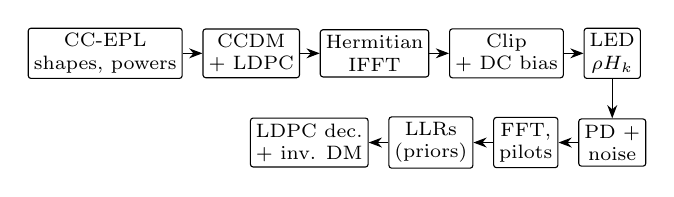
\begin{tikzpicture}[node distance=2.5mm,box/.style={draw,rounded corners=1pt,minimum height=6mm,align=center,font=\scriptsize,inner sep=2pt},>=Stealth]
\node[box](ld){CC-EPL\\shapes, powers};
\node[box,right=of ld](dm){CCDM\\+ LDPC};
\node[box,right=of dm](ifft){Hermitian\\IFFT};
\node[box,right=of ifft](cl){Clip\\+ DC bias};
\node[box,right=of cl](led){LED\\$\rho H_k$};
\node[box,below=5mm of led](pd){PD +\\noise};
\node[box,left=of pd](fft){FFT,\\pilots};
\node[box,left=of fft](llr){LLRs\\(priors)};
\node[box,left=of llr](dec){LDPC dec.\\+ inv. DM};
\draw[->](ld)--(dm);\draw[->](dm)--(ifft);\draw[->](ifft)--(cl);\draw[->](cl)--(led);\draw[->](led)--(pd);
\draw[->](pd)--(fft);\draw[->](fft)--(llr);\draw[->](llr)--(dec);
\end{tikzpicture}}
\caption{DCO-OFDM link with CC-EPL and the PAS chain used in the coded evaluation.}\label{fig:block}
\end{figure}

\section{Re-examination of the Base Paper}\label{sec:repro}
We implemented eqs.~(4)--(16) and Algorithms~1--2 of~\cite{pham2026} with its parameters and evaluated the mutual information with $24\times24$-point Gauss--Hermite quadrature.

\textit{Clipping-noise variance.} The printed eq.~(9) of~\cite{pham2026} defines $\phi(t)=e^{-t^2/2}/(2\pi)$. The terms of~\eqref{eq:clip} are moments of a clipped Gaussian; for example, for $x\sim\mathcal N(0,\sigma_x^2)$,
\begin{equation}
\mathbb{E}\big[x\,\mathbf 1\{x>\beta\sigma_x\}\big]=\frac{\sigma_x}{\sqrt{2\pi}}\int_\beta^\infty t\,e^{-t^2/2}\,dt=\sigma_x\,\phi(\beta),
\end{equation}
which holds only when $\phi$ is the standard normal density, i.e.\ the same density whose tail defines $Q(t)=\int_t^\infty\phi(u)\,du$ in~\eqref{eq:clip}. With the printed normalization, $\int\phi(t)\,dt=1/\sqrt{2\pi}\approx0.40$, so $\phi$ is not a density and is inconsistent with the $Q$-function in the same expression. Table~\ref{tab:mc} compares both forms with a Monte Carlo estimate from $2\times10^6$ clipped Gaussian samples: the standard normal pdf in~\eqref{eq:clip} matches to within 0.4\,\%, while the printed form overestimates $\sigma^2_{\mathrm{clip}}$ by 6--13 times.
% TODO (author): state the random seed / number of independent runs used for Table II.

\begin{table}[t]\centering\footnotesize
\caption{Clipping-noise variance (mA$^2$): Monte Carlo vs.\ eq.~(9)}\label{tab:mc}
\begin{tabular}{@{}rrrr@{}}\toprule
$\sigma_x$ (mA) & Monte Carlo & Eq.~(9), $1/\sqrt{2\pi}$ & Eq.~(9) as printed \\\midrule
221 & 500 & 500 & 6659 (13.3$\times$) \\
394 & 7192 & 7166 & 51013 (7.1$\times$) \\
700 & 23334 & 23329 & 145879 (6.3$\times$) \\
1245 & 40622 & 40622 & 292248 (7.2$\times$) \\
\bottomrule\end{tabular}\end{table}


\textit{Capacity.} Fig.~\ref{fig:repro} and Table~\ref{tab:cap} show 16-QAM capacity on the flat channel. With the correct model the best PCS on the paper's fixed grid gains \PCSgainCorrect\,\% over uniform signaling at full power at 15\,dB ($2.729$ vs.\ $2.254$\,bit); with the printed pdf the gain is 67--90\,\% between 10 and 20\,dB, bracketing the reported 72.6\,\%. Because the code of~\cite{pham2026} is not public, this is consistent with, but does not prove, an implementation of the printed form.

\textit{Missing baseline.} The comparison in~\cite{pham2026} is against uniform signaling at full power. Scaling the uniform constellation to the best power gives \BackoffCap\,bit at 15\,dB, more than the paper's PCS (\PCSCap\,bit): on a fixed grid PCS can only back off indirectly, by moving probability to inner points at the cost of entropy.

\textit{Optimizer.} We implemented Algorithm~1 as printed, with the published step $\tau=10^{-4}$ and tolerance $\varepsilon=10^{-3}$. In our implementation the relative-change stopping test is met after one iteration at 5 and 15\,dB, so the returned distribution is practically uniform. This concerns the printed settings only; since the authors' code is not public, we cannot tell whether their implementation used different values. With a larger fixed step ($\tau=0.05$) the iterates cycle between a few points, and the result depends on when the loop stops. With step-size control (a step is accepted only if it increases $C(\mathbf{p})$), PGD converged in 20--80 iterations in our runs to \PGDconv\,bit at 15\,dB, the same value as the best MB distribution. In our tests, therefore, the algorithm behaves well once its step size is controlled; this is an empirical observation, not a proof of convergence or global optimality. The printed update is also written as a descent step although the problem is a maximization; we used the ascent direction.
% TODO (author): state the initial distribution used for Algorithm 1.

\begin{table}[t]\centering\footnotesize
\caption{16-QAM capacity (bit/symbol), flat channel}\label{tab:cap}
\begin{tabular}{@{}rrrrrr@{}}\toprule
$E_b/N_0$ & Uniform & PCS~\cite{pham2026} & Gain & Back-off & Gain, printed \\\midrule
5 & 3.181 & 3.190 & +0.3\,\% & 3.181 & +15.9\,\% \\
10 & 2.914 & 3.228 & +10.8\,\% & 3.241 & +66.9\,\% \\
15 & 2.254 & 2.729 & +21.1\,\% & 3.242 & +89.9\,\% \\
20 & 1.859 & 2.229 & +19.9\,\% & 3.242 & +90.5\,\% \\
\bottomrule\end{tabular}
\vspace{1mm}\\\footnotesize Paper reports +72.6\,\% at 15\,dB.\end{table}


\begin{figure}[t]\centering
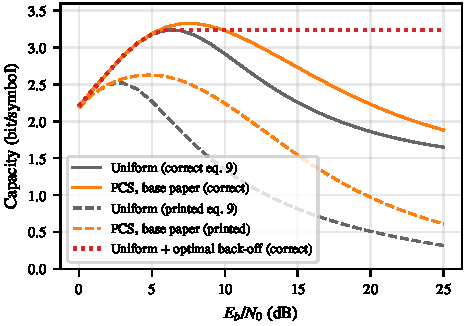
\includegraphics[width=\columnwidth]{figures/fig_reproduction.pdf}
\caption{Re-implementation of~\cite{pham2026} (16-QAM, flat channel): correct vs.\ printed clipping-noise variance, and uniform signaling with optimal back-off.}\label{fig:repro}
\end{figure}

\section{Clipping-Coupled Entropy-and-Power Loading}\label{sec:ccepl}
\subsection{Problem}
Let each subcarrier use an MB distribution $p_k(x)\propto e^{-\nu_k|x|^2}$ on the 16-QAM grid scaled to power $E_k$. We maximize the sum mutual information
\begin{equation}
\max_{\{\nu_k,E_k\}}\sum_{k=1}^{K} I_{\nu_k}\!\big(\mathrm{SNR}_k\big)\quad \text{s.t.}\quad \sum_k E_k\le KP, \label{eq:prob}
\end{equation}
where $\mathrm{SNR}_k$ is~\eqref{eq:snr} and $I_\nu(\cdot)$ is the mutual information of shape $\nu$ in AWGN. Every $\mathrm{SNR}_k$ depends on all $E_j$ through $\sigma_x$, so~\eqref{eq:prob} is coupled and non-convex; prior entropy loading~\cite{ding2020,ma2026,song2024} ignores this dependence, and~\cite{pham2026} restricts it to $\nu_k=\nu$, $E_k=P\,\mathbb{E}_\nu|x|^2$.

\begin{proposition}\label{prop:dec}
Problem~\eqref{eq:prob} equals $\max_{0<\Sigma\le KP} F(\Sigma)$ with
\begin{equation}
F(\Sigma)=\max_{\{\nu_k,E_k\}:\sum_k E_k=\Sigma}\ \sum_k I_{\nu_k}\!\big(g_k(\Sigma)E_k\big),
\end{equation}
where $g_k(\Sigma)=\rho^2|H_k|^2R^2/(\rho^2|H_k|^2\sigma^2_{\mathrm{clip}}+\sigma_z^2)$ is evaluated at $\sigma_x=\sqrt{2\Sigma/N}$. For fixed $\Sigma$ the inner problem is separable with a single linear constraint.
\end{proposition}
\begin{proof}
Under the Gaussian model of Section~\ref{sec:model}, $R$ and $\sigma^2_{\mathrm{clip}}$ depend on the allocation only through $\sigma_x^2=2\Sigma/N$. Partitioning the feasible set of~\eqref{eq:prob} by the value of $\Sigma=\sum_kE_k$ fixes $g_k$ on each part, which gives the stated nested form; the objective then splits over $k$.
\end{proof}

By Proposition~\ref{prop:dec}, the inner problem can be solved through its Lagrangian: for a multiplier $\lambda$ each subcarrier independently maximizes $I_{\nu}(g_kE)-\lambda E/P$ over a table of shapes and powers, and bisection on $\lambda$ meets $\sum_kE_k=\Sigma$. We have not proved that the duality gap of this discrete inner problem is zero. For separable problems with many subcarriers the gap is usually small (a time-sharing argument), and we use the Lagrangian solution as an approximation. Because each final allocation is re-scored exactly (line~7 of Algorithm~\ref{alg}), a non-zero gap can only make CC-EPL sub-optimal; it cannot inflate its reported rate. The outer problem is a scalar search over $\Sigma$ (Algorithm~\ref{alg}).

\begin{algorithm}[t]\caption{CC-EPL}\label{alg}\small
\begin{algorithmic}[1]
\State Offline: table $T[\nu,\mathrm{SNR}]=I_\nu(\mathrm{SNR})$ for 24 MB shapes, $-15$ to $45$\,dB
\For{$\Sigma$ on a log grid in $(0,KP]$}
\State $\sigma_x\gets\sqrt{2\Sigma/N}$; compute $R,\sigma^2_{\mathrm{clip}}$ by~\eqref{eq:clip}; $g_k$ for all $k$
\Repeat \Comment{bisection on $\lambda$}
\State $(\nu_k,E_k)\gets\arg\max_{\nu,E}\,T[\nu,g_kE]-\lambda E/P$ for all $k$
\Until{$\sum_kE_k=\Sigma$}
\State score $\sum_k T[\nu_k,\mathrm{SNR}_k]$ with $\sigma_x$ recomputed from $\{E_k\}$
\EndFor
\State \Return best allocation
\end{algorithmic}\end{algorithm}

\textit{Complexity.} With 40 outer points, 50 bisection steps, 24 shapes, 160 power levels and $K=63$ subcarriers the algorithm performs $40\cdot50\cdot24\cdot160\cdot63\approx4.8\times10^{8}$ table look-ups (an operation count, not a measured quantity). In vectorized NumPy this took under 3\,s on our machine.
% TODO (author): name the CPU / Python and NumPy versions used for this timing. No gradient or non-convex solver is involved. Restricting the shapes to the uniform one recovers clipping-aware power loading in the spirit of~\cite{ling2020}, which we use as the strongest baseline.

\section{Practical PAS Implementation}\label{sec:pas}
To verify that the information-theoretic gains survive practical coding, we implement PAS for 16-QAM as two 4-PAM dimensions with Gray labels (sign bit, amplitude bit). The MB shape of subcarrier $k$ fixes $P(|x|=3)$ per real dimension; a binary CCDM with exact enumerative ranking maps $\lfloor\log_2\binom{n}{w}\rfloor$ data bits to a length-$n=256$ amplitude sequence with $w$ outer amplitudes. One codeword of an irregular repeat-accumulate (IRA) LDPC code ($N_c=32256$, linear-time encoding, normalized min-sum with 50 iterations) spans a frame of 128 data OFDM symbols. Amplitude bits are systematic and randomly interleaved over the frame; signs carry the remaining data bits and the parity, also interleaved. All schemes share one code library: for every rate, DVB-S2-style information-node profiles with 20\,\% degree-8 nodes (other nodes degree 3), and, for rates up to 0.55, denser profiles with 30--40\,\% degree-12 nodes; each scheme uses the best rate/profile pair. Uniform schemes use the same bit placement and may also use rates below 1/2.

Each frame carries 16 QPSK pilot symbols for least-squares gain and noise estimation, the signal is clipped in the time domain, and the receiver computes bit LLRs including the amplitude priors. For each scheme and $E_b/N_0$ the code rate is chosen from 0.3--0.9 (step 0.025) to maximize goodput $=$ information bits $\times(1-\mathrm{FER})$ per frame time over 40 frames.

\section{Results}\label{sec:results}
\subsection{Analytical comparison}
Fig.~\ref{fig:sweep} compares six schemes and the Gaussian bound; Table~\ref{tab:main} lists the values at 15\,dB. The base paper's single distribution peaks near 10\,dB and decays as clipping grows; uncoupled entropy loading measures the SNR at full power and loads the full budget, so it stays in heavy clipping and falls \emph{below} the base paper. Schemes that select the operating point stay flat. In this analytical model CC-EPL is \GainPOmin--\GainPOmax\,\% above coupled power loading~\cite{ling2020} at every tested channel and $E_b/N_0$, reaching \BoundMin--\BoundMax\,\% of the Gaussian bound. At 15\,dB on the 5\,MHz LED, CC-EPL uses only \CCpower\,\% of the power budget and spreads the subcarrier entropies over \EntMin--\EntMax\,bit (Fig.~\ref{fig:alloc}).

\begin{figure*}[t]\centering
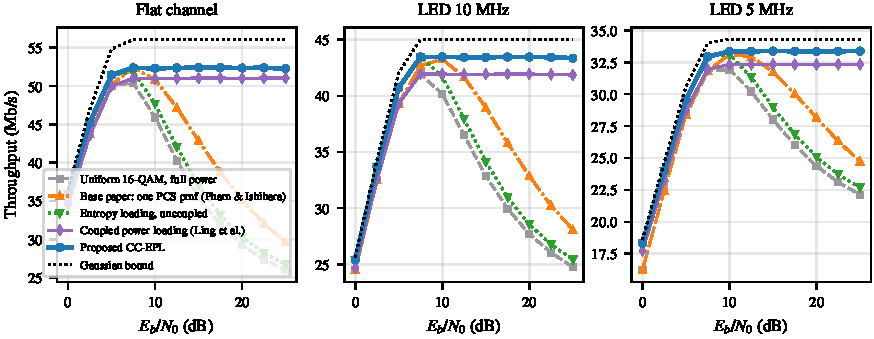
\includegraphics[width=\textwidth]{figures/fig_sweep.pdf}
\caption{Analytical throughput vs.\ $E_b/N_0$ for a flat channel and low-pass LEDs with 10 and 5\,MHz bandwidth.}\label{fig:sweep}
\end{figure*}

\begin{table}[t]\centering\footnotesize
\caption{Analytical throughput (Mb/s) at $E_b/N_0=15$\,dB}\label{tab:main}
\begin{tabular}{@{}lrrr@{}}\toprule
Scheme & Flat & LED 10\,MHz & LED 5\,MHz \\\midrule
Uniform 16-QAM, full power & 35.50 & 32.89 & 28.01 \\
Entropy loading, uncoupled & 37.02 & 34.13 & 28.99 \\
Base paper, one PCS pmf~\cite{pham2026} & 42.88 & 38.96 & 31.74 \\
Uniform + optimal back-off & 51.05 & 41.94 & 32.21 \\
Coupled power loading~\cite{ling2020} & 51.05 & 41.93 & 32.33 \\
\textbf{CC-EPL (proposed)} & \textbf{52.40} & \textbf{43.44} & \textbf{33.37} \\
Gaussian bound & 56.11 & 45.03 & 34.29 \\
\midrule
CC-EPL vs.~\cite{pham2026} & +22.2\,\% & +11.5\,\% & +5.1\,\% \\
CC-EPL vs.~\cite{ling2020} & +2.6\,\% & +3.6\,\% & +3.2\,\% \\
\bottomrule\end{tabular}\end{table}


\subsection{Waveform-level validation}
The Bussgang model assumes a Gaussian time-domain signal and Gaussian, independent clipping noise. We transmitted 4000 OFDM symbols per point with actual clipping and estimated gain and noise per subcarrier from the data. Fig.~\ref{fig:val} shows that the achievable rate of a Gaussian mismatched decoder agrees with the analytical value to within \ValMaxDev\,\% for all 48 combinations of scheme, channel and $E_b/N_0$; the mean SNR deviation is \ValSNRmin--\ValSNRmax\,dB, and the ranking of the schemes is unchanged.

\begin{figure}[t]\centering
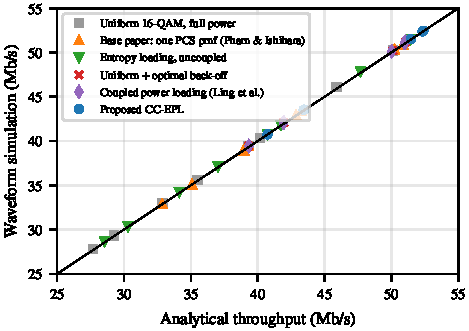
\includegraphics[width=\columnwidth]{figures/fig_validation.pdf}
\caption{Time-domain simulation with real clipping vs.\ analytical throughput (flat and 10\,MHz LED, $E_b/N_0=5$--$20$\,dB).}\label{fig:val}
\end{figure}

\subsection{Coded goodput}
Fig.~\ref{fig:coded} and Table~\ref{tab:coded} show the goodput we measured with the full coded chain. CC-EPL gives the highest goodput at 8 of the 8 operating points. From 10\,dB upwards it is 3.6--5.3\,\% ahead of coupled power loading with uniform 16-QAM~\cite{ling2020} and 1.5--55.3\,\% ahead of the base paper~\cite{pham2026}. The goodput is 83--90\,\% of the mutual-information bound after pilot overhead; the rest is lost to the LDPC code, the 0.025 step in code rate and the rate loss of the distribution matcher. The schemes rank in the same order as in the analysis. The coded margin over~\cite{ling2020} is a little larger than the analytical one, probably because the distribution matcher can adjust the rate in small steps while uniform QAM is limited to the code-rate grid. To check that this margin is not a seed artefact, we repeated the 10\,MHz LED points with 80 new frames at the chosen rate and one step above. The ranking is the same, but the margin over~\cite{ling2020} shrinks to 1.3--2.6\,\%, because in the first run the baseline lost one frame out of 40. We therefore quote the coded margin over~\cite{ling2020} as roughly 1--5\,\%.


\begin{figure}[t]\centering
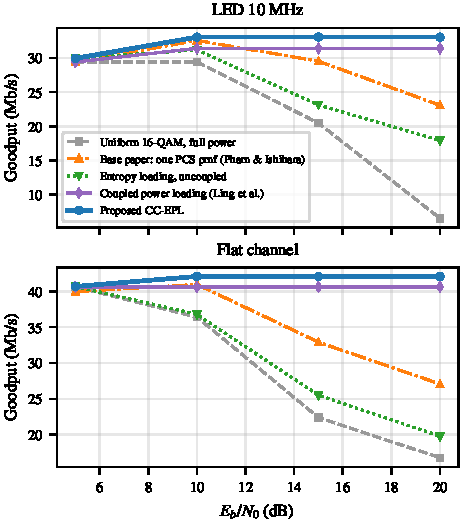
\includegraphics[width=\columnwidth]{figures/fig_coded.pdf}
\caption{Measured goodput with CCDM, irregular LDPC codes and pilot-based estimation (time-domain clipping).}\label{fig:coded}
\end{figure}

\begin{table}[t]\centering\footnotesize
\caption{Measured coded goodput (Mb/s), 40 frames per code rate, pilot overhead included}\label{tab:coded}
\begin{tabular}{@{}lrrrrrr@{}}\toprule
Ch. & $E_b/N_0$ & Uni. & \cite{pham2026} & Unc.\ EL & \cite{ling2020} & CC-EPL \\\midrule
LED & 5 & 29.4 & 29.4 & 29.9 & 29.4 & \textbf{29.9} \\
LED & 10 & 29.4 & 32.6 & 31.2 & 31.4 & \textbf{33.0} \\
LED & 15 & 20.5 & 29.5 & 23.1 & 31.4 & \textbf{33.1} \\
LED & 20 & 6.5 & 23.1 & 17.9 & 31.4 & \textbf{33.0} \\
Flat & 5 & 40.6 & 39.9 & 40.7 & 40.6 & \textbf{40.7} \\
Flat & 10 & 36.4 & 40.9 & 36.8 & 40.6 & \textbf{42.1} \\
Flat & 15 & 22.4 & 32.9 & 25.5 & 40.6 & \textbf{42.1} \\
Flat & 20 & 16.8 & 27.1 & 19.8 & 40.6 & \textbf{42.1} \\
\bottomrule\end{tabular}\end{table}


\subsection{Robustness}
Fig.~\ref{fig:rob}(a) shows the mean throughput over 5--20\,dB on the 10\,MHz LED when CC-EPL may use only $K$ shapes chosen by greedy selection: two shapes reach \KtwoPct\,\% and three shapes \KthreePct\,\% of the full 24-shape set, so the distribution-matcher cost is small. Fig.~\ref{fig:rob}(b) shows that misjudging $\sigma_x$ by $\pm30$\,\% costs at most \MisMax\,\%, and CC-EPL still exceeds the exact coupled power loading. Fig.~\ref{fig:rob}(c) shows that the gain over~\cite{pham2026} grows with LED bandwidth while the gain over~\cite{ling2020} stays at 2.6--3.6\,\%.

\begin{figure*}[t]\centering
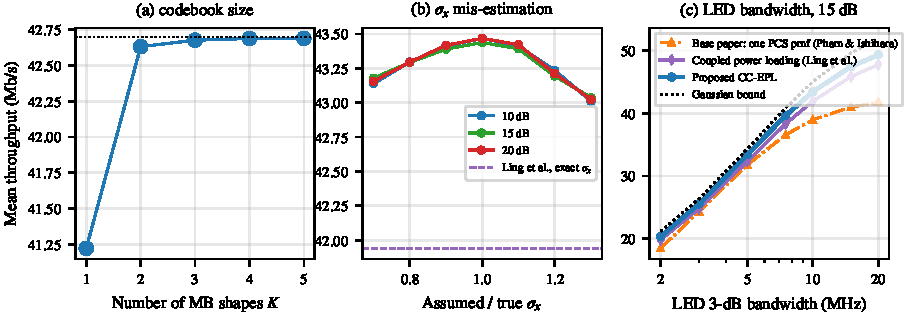
\includegraphics[width=\textwidth]{figures/fig_robustness.pdf}
\caption{Robustness of CC-EPL (10\,MHz LED unless stated): (a) number of shapes, (b) mis-estimated operating point, (c) LED bandwidth at 15\,dB.}\label{fig:rob}
\end{figure*}

\begin{figure}[t]\centering
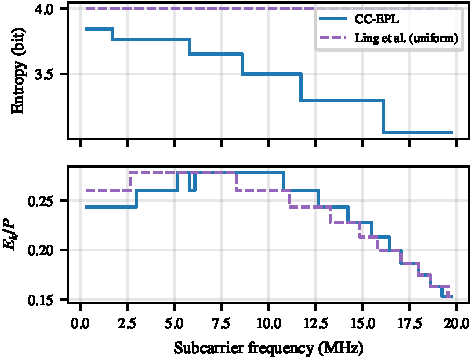
\includegraphics[width=\columnwidth]{figures/fig_allocation.pdf}
\caption{Allocation at 15\,dB on the 5\,MHz LED: CC-EPL vs.\ coupled power loading with uniform 16-QAM.}\label{fig:alloc}
\end{figure}

\section{Circuit-Level Co-Simulation with ngspice}\label{sec:spice}
The analysis so far, like the base paper, treats the transmitter as an ideal clipper followed by a linear LED. To test the conclusions with a less idealized transmitter and receiver, we co-simulated the link at circuit level with ngspice~42, the SPICE engine that KiCad also uses. This is a circuit simulation, not a hardware measurement: the LED is a behavioural model with generic parameters. Python generates the OFDM waveforms and does all receiver processing; ngspice simulates the circuit of Fig.~\ref{fig:schem}:
\begin{itemize}
\item a zero-order-hold DAC with a 60\,MHz reconstruction pole and a transconductance LED driver with a compliance knee;
\item the LED as a diode with a carrier rate equation ($\tau=15.9$\,ns, i.e.\ 10\,MHz modulation bandwidth) and efficiency droop $P=\eta_0 I/(1+I/3\,\mathrm{A})$, with $\eta_0$ chosen so that the slope at the 500\,mA bias equals the base paper's $\eta=0.44$\,W/A;
\item a photodiode with 5\,pF capacitance, white receiver noise with the base paper's $N_0$ injected at the photodiode, and a transimpedance amplifier ($R_f=10$\,k$\Omega$, op-amp GBW 1\,GHz).
\end{itemize}
The receiver applies an anti-alias filter with a smooth, power-complementary roll-off between $0.9B$ and $1.1B$, recovers the timing blindly (coarse alignment by correlation, then the sampling phase with maximum output power), samples at 40\,MSa/s and estimates gain and noise from the received data, so nothing about the circuit is assumed. Each scheme is given the channel magnitude from an ngspice AC analysis multiplied by the DAC sinc, as it would obtain from channel sounding.

We calibrated the link first: without clipping and droop, the measured subcarrier SNR matches the AC prediction (times the DAC sinc) to within 0.12\,dB on average; below $0.9B$ the gains agree to 2.9\,\% and the noise is 1.06 times $BN_0$, while the top subcarriers are reshaped by the receiver filter and sampling phase (their SNR comes out about 1.3\,dB above the simple prediction).

\begin{figure*}[t]\centering
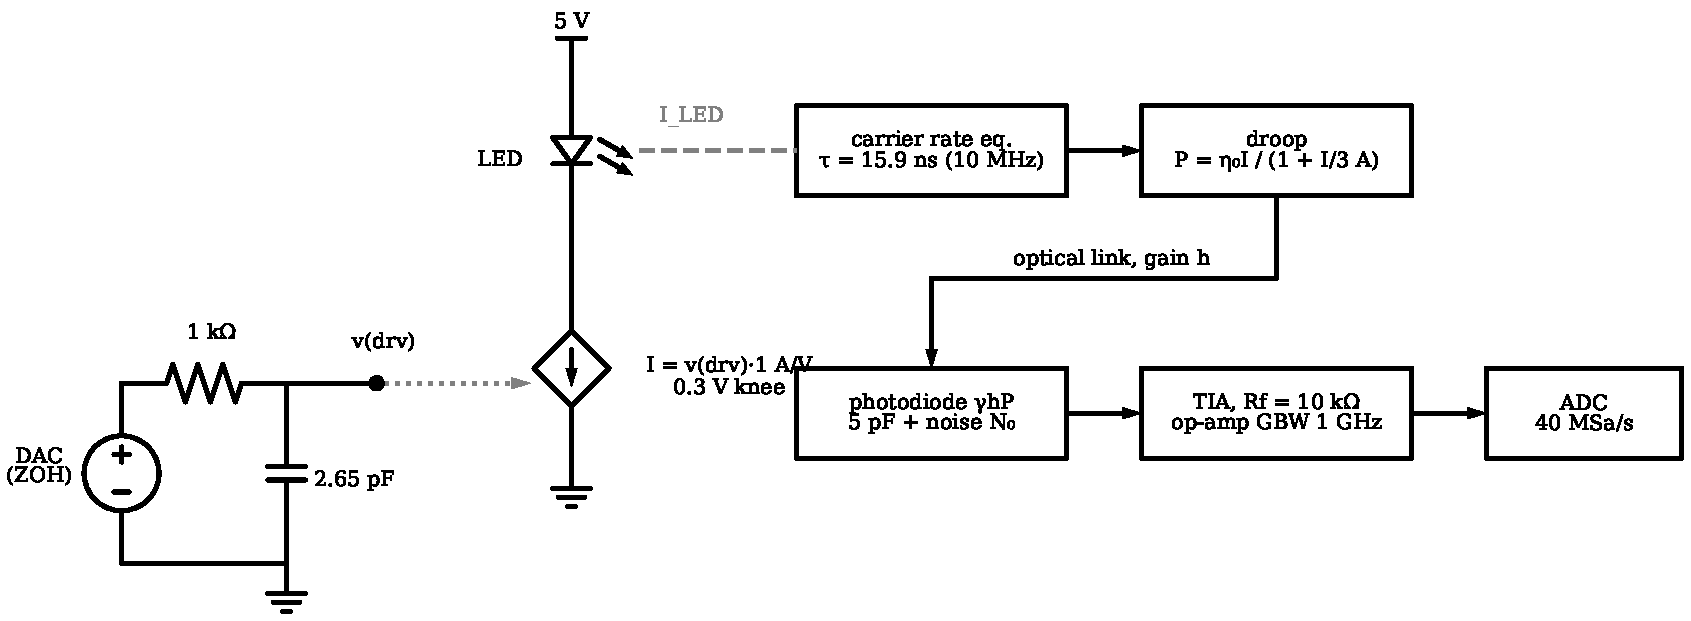
\includegraphics[width=0.82\textwidth]{figures/fig_schematic.pdf}
\caption{Optical front end simulated in ngspice. The LED optical model and the receiver are behavioural sources in the same netlist.}\label{fig:schem}
\end{figure*}

We ran \SpRuns\ cases (two circuits, five values of $E_b/N_0$, seven schemes, 400 OFDM symbols each). Besides the stronger single-distribution variant used so far, the base paper is now also represented by its own Algorithm~1 (step-controlled PGD on its flat-channel objective). Through the circuit the throughput is at most \SpLossMax\,\% below the analytical model (which already includes the DAC sinc in the channel; one point is \SpOver\,\% above it, within the estimation noise), and droop costs a further \SpDroopMin--\SpDroopMax\,\% (Fig.~\ref{fig:spice}). The ranking does not change: CC-EPL is the best scheme, or within 0.05\,\% of the best, at all \SpCases\ circuit operating points. Through the circuit with droop it gains \SpPOmin--\SpPOmax\,\% over coupled power loading and \SpBaseMin--\SpBaseMax\,\% over Algorithm~1 of the base paper (Table~\ref{tab:spice}); the small value is at 10\,dB, where clipping is mild and one distribution is close to optimal.

\begin{figure*}[t]\centering
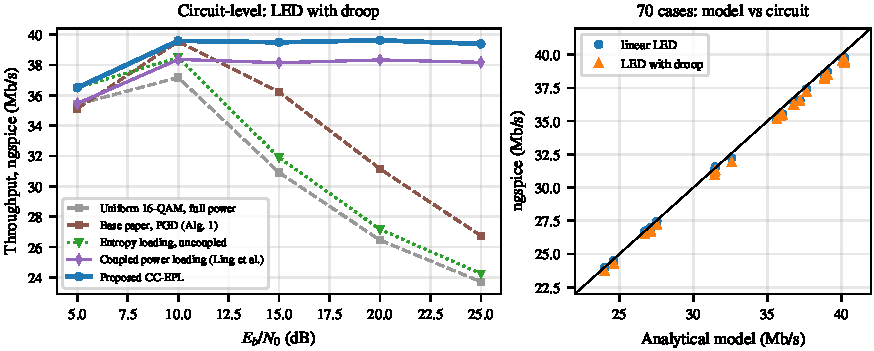
\includegraphics[width=\textwidth]{figures/fig_spice.pdf}
\caption{Left: throughput through the ngspice circuit with LED droop. Right: analytical model vs.\ circuit for all \SpRuns\ cases.}\label{fig:spice}
\end{figure*}

\begin{table}[t]\centering\footnotesize
\caption{Throughput (Mb/s) through the ngspice circuit, LED with droop}\label{tab:spice}
\begin{tabular}{@{}lrrrr@{}}\toprule
Scheme \;/\; $E_b/N_0$ & 10\,dB & 15\,dB & 20\,dB & 25\,dB \\\midrule
Uniform 16-QAM, full power & 37.17 & 30.91 & 26.46 & 23.71 \\
Base paper, Alg.~1 (PGD) & 39.54 & 36.21 & 31.15 & 26.74 \\
Base paper, best MB pmf & 39.52 & 36.20 & 31.29 & 26.62 \\
Entropy loading, uncoupled & 38.48 & 31.90 & 27.17 & 24.25 \\
Coupled power loading~\cite{ling2020} & 38.36 & 38.14 & 38.32 & 38.17 \\
\textbf{CC-EPL} & \textbf{39.58} & \textbf{39.48} & \textbf{39.62} & \textbf{39.37} \\
\midrule CC-EPL vs Alg.~1 & +0.1\,\% & +9.0\,\% & +27.2\,\% & +47.3\,\% \\
CC-EPL vs~\cite{ling2020} & +3.2\,\% & +3.5\,\% & +3.4\,\% & +3.2\,\% \\
\bottomrule\end{tabular}\end{table}


\IfFileExists{tables/spice_coded_text.tex}{Table~\ref{tab:spicecoded} repeats the coded test of Section~\ref{sec:results} through the circuit with droop, 12 frames per code rate. Relative to the base paper's Algorithm~1, CC-EPL delivers +7.4\,\% (15\,dB) and +45.5\,\% (20\,dB) goodput, and relative to coupled power loading -0.7\,\% and +4.4\,\%. At 15\,dB coupled power loading is marginally ahead, which is within the resolution of this test: with only 12 frames per rate and a 0.025 code-rate grid these coded figures are less precise than the analytical ones; the analytical ngspice comparison above (400 symbols per point) keeps CC-EPL ahead at every point.
\begin{table}[t]\centering\footnotesize
\caption{Coded goodput (Mb/s) through the ngspice circuit (code rate in brackets), 12 frames per rate}\label{tab:spicecoded}
\begin{tabular}{@{}lrr@{}}\toprule
Scheme & 15\,dB & 20\,dB \\\midrule
Base paper, Alg.~1 & 25.9 (0.650) & 20.1 (0.675) \\
Base paper, best MB & 26.7 (0.725) & 20.1 (0.675) \\
Coupled power~\cite{ling2020} & 28.0 (0.500) & 28.0 (0.500) \\
\textbf{CC-EPL} & \textbf{27.8} (0.600) & \textbf{29.2} (0.625) \\
\bottomrule\end{tabular}\end{table}
}{}

\section{The OFDM Ceiling}\label{sec:ceiling}
CC-EPL reaches \BoundMin--\BoundMax\,\% of the Gaussian-input bound for clipped DCO-OFDM (Table~\ref{tab:main}), so within this model a better OFDM shaping or loading rule could add at most about 7\,\%. The bound is set by the clipping noise, and this section examines how far the shaping can influence that noise.

\begin{proposition}\label{prop:clt}
Let the subcarrier symbols $X_k$ be independent with powers $E_k$ and arbitrary distributions on a bounded constellation. If $\max_k E_k/\sum_k E_k\to 0$, each time sample $x[n]$ of the DCO-OFDM symbol converges in distribution to $\mathcal{N}(0,\sigma_x^2)$, $\sigma_x^2=\frac{2}{N}\sum_kE_k$, so $R$ and $\sigma^2_{\mathrm{clip}}$ in~\eqref{eq:clip} depend on the distributions only through the powers.
\end{proposition}
\begin{proof}
$x[n]=\frac{2}{\sqrt N}\sum_k\Re\{X_ke^{j2\pi kn/N}\}$ is a sum of independent, zero-mean, bounded terms with variances $E_k/N$ (per term and real dimension); the condition is Lindeberg's.
\end{proof}

Proposition~\ref{prop:clt} is a large-$N$ result. For the $N=128$ used here we checked it numerically: drawing 4000 OFDM symbols with uniform 16-QAM and with MB shapes ($\nu=0.1$ and $0.3$) at the same power changes the clipping-distortion variance by at most \ClipShapeDev\,\% at 10, 15 and 20\,dB. In this model, shaping therefore affects clipping mainly by lowering the power, which a power back-off also does (Section~\ref{sec:repro}). Within DCO-OFDM, the subcarrier distributions cannot directly control how the signal uses the LED current range.

\textit{Can the receiver recover the clipping?} Clipping is a deterministic function of the data, so a turbo receiver could in principle rebuild it from decoder feedback. We built such a receiver on a conditional Bussgang model: given the decoder's soft estimate $\hat x[n]$ and the error variance $\varepsilon$ (Gaussian by the same CLT argument), the clipped sample has a closed-form mean, variance and gain, and subtracting the predicted clipping leaves $R\,X_k$ plus a residual that is uncorrelated with $X_k$. With no a-priori information this is exactly~\eqref{eq:bussgang}; with perfect information only thermal noise remains.

Fig.~\ref{fig:exit} shows the EXIT curves of this demapper for four drive levels. The extrinsic information rises appreciably only once the a-priori information is already high. The area under each curve, which bounds the rate a matched code could reach, is therefore at most \ExitGain\,\% above the starting point (\ExitArea\ vs.\ \ExitIE). Heavier drive does not help, because it lowers the starting point faster than it raises the end point. In this model, most of the loss caused by clipping could not be recovered by the decoder-aided receiver we tested.

\begin{figure}[t]\centering
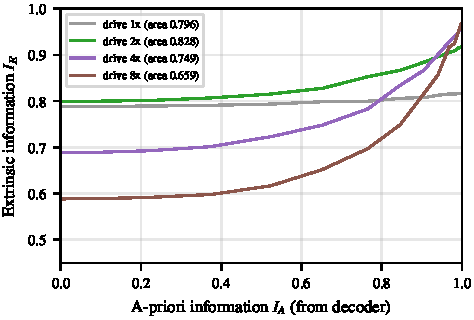
\includegraphics[width=\columnwidth]{figures/fig_exit.pdf}
\caption{EXIT curves of decoder-aided clipping recovery (flat channel, uniform 16-QAM, drive relative to $E_b/N_0=5$\,dB).}\label{fig:exit}
\end{figure}

\begin{figure*}[t]\centering
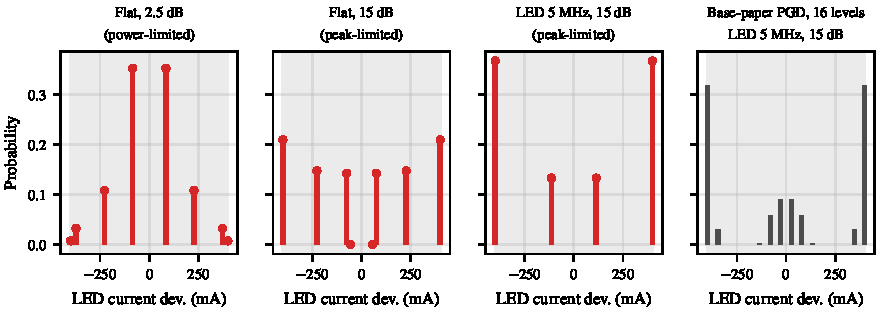
\includegraphics[width=\textwidth]{figures/fig_pm_shapes.pdf}
\caption{PM-PCS constellations (positions in mA from the bias, probabilities). Grey band: LED range. Right: the base paper's PGD with the peak-matched objective on a 16-level grid.}\label{fig:shapes}
\end{figure*}

\begin{figure*}[t]\centering
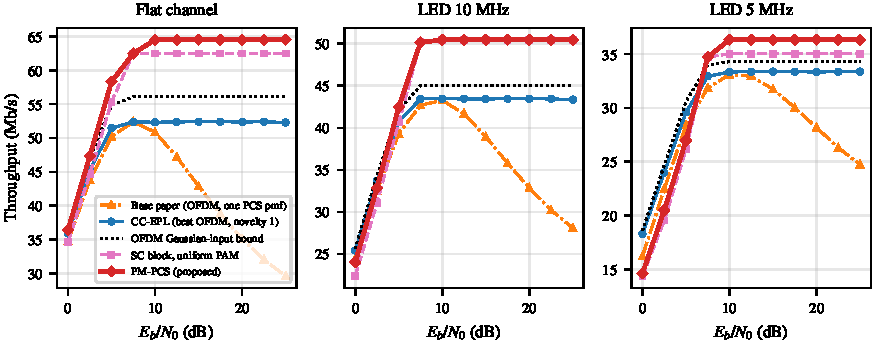
\includegraphics[width=\textwidth]{figures/fig_pm_sweep.pdf}
\caption{Analytical throughput: OFDM schemes (base paper, CC-EPL, OFDM Gaussian bound) and single-carrier blocks with uniform PAM and with PM-PCS.}\label{fig:pmsweep}
\end{figure*}

\section{Peak-Matched Probabilistic Shaping}\label{sec:pmpcs}
\subsection{Idea}
When the time-domain waveform is approximately Gaussian, the subcarrier distributions have little control over its peaks. When each time sample is a constellation point, the peak of the constellation is the peak of the waveform, and the constellation's distribution determines how the LED range is used. This is what a DFT-spread block does: spreading the $N$ real samples of a block over all bins and taking the inverse transform returns the samples themselves, so the transmitter sends $N=128$ PAM-like samples per block with the same cyclic prefix, sample rate and bandwidth as the OFDM link, and the receiver equalizes in the frequency domain with the same FFT (Fig.~\ref{fig:wave}). The LED range $[I_{\min},I_{\max}]$ becomes a hard constraint on the constellation, $|x|\le A=400$\,mA around the 500\,mA bias (the extra 100\,mA headroom above the bias is not used), and there is no clipping: in Fig.~\ref{fig:wave} the OFDM signal is approximately Gaussian and must be clipped, whereas the PM-PCS signal stays inside the range by construction. The average-power budget is the same as for OFDM, $\mathbb{E}x^2\le 2KP/N$.

\begin{figure}[t]\centering
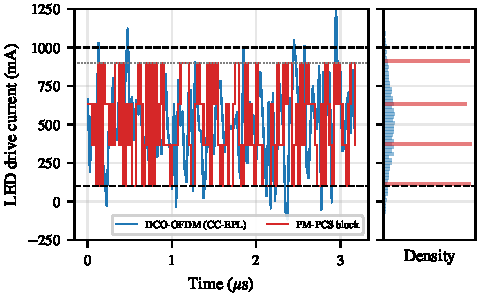
\includegraphics[width=\columnwidth]{figures/fig_waveforms.pdf}
\caption{LED drive current for one block (10\,MHz LED, 15\,dB): DCO-OFDM at CC-EPL's operating point (blue, before clipping; dashed: LED range) and PM-PCS (red). Right: amplitude histograms.}\label{fig:wave}
\end{figure}

\subsection{Rate model and optimization}
With a minimum mean-square-error frequency-domain equalizer, the unbiased SINR of every sample is
\begin{equation}
\mathrm{SINR}=\Big(\frac1N\sum_{k=0}^{N-1}\frac{1}{1+\rho^2|H_k|^2P_s/\sigma_z^2}\Big)^{-1}-1,\label{eq:sinr}
\end{equation}
where $P_s$ is the signal power. Because the coded system feeds bit LLRs to an LDPC decoder, we use the bit-metric rate of PAS with Gray labels, $R_{\mathrm{BMD}}=H(X)-\sum_bH(B_b\,|\,Y)$~\cite{bocherer2023}, evaluated by Gauss--Hermite quadrature at the SINR of~\eqref{eq:sinr}. A constellation is symmetric with $M\in\{4,8\}$ points at positions $\pm A u_i$, $0<u_1<\dots<u_{M/2}=1$, and probabilities $q_i$. PM-PCS solves
\begin{equation}
\begin{aligned}
\max_{\mathbf u,\mathbf q,M}\ & R_{\mathrm{BMD}}(\mathbf u,\mathbf q)\\
\text{s.t.}\ & A^2\textstyle\sum_i q_iu_i^2\le 2KP/N,\quad H(|X|)\le R_{\mathrm{BMD}}-\delta,
\end{aligned}\label{eq:pmprob}
\end{equation}
where the last constraint keeps the constellation codable by PAS (all amplitude bits are sent systematically, so the code cannot carry less than $H(|X|)$; $\delta=0.3$\,bit allows for the gap of a practical code). We solve~\eqref{eq:pmprob} by a multi-start Nelder--Mead search; equally spaced uniform and MB constellations are included as candidates, and candidates are compared after subtracting the rate loss of a length-384 distribution matcher. For fixed equally spaced positions the problem in $\mathbf q$ alone is the base paper's: maximize a rate over the probability simplex under a linear power constraint. We therefore also ran Algorithms~1--2 of~\cite{pham2026} (with step control) on a dense 16-level grid; only the objective changes, from the clipped-OFDM capacity to the peak-matched rate.

\subsection{What the optimal inputs look like}
Fig.~\ref{fig:shapes} and Table~\ref{tab:pmshapes} show the result. At low $E_b/N_0$ the power budget binds and the optimum is MB-like, with most probability on the inner points, which is the base paper's intuition. Once the LED range binds, probability moves to the outer points: on the 5\,MHz LED at 15\,dB the outer points carry probability 0.73, and on the flat channel the 8-point constellation degenerates to six used points. The base paper's own PGD, run on the dense grid (right panel), concentrates the probability on a few levels and leaves most of the grid empty; this is the discrete, few-mass-point structure that the theory of amplitude-constrained channels predicts~\cite{dytso2020}. The appropriate shaping therefore depends on which constraint is active; in the regime where clipped OFDM saturates, the optimized inputs found here are not Maxwell--Boltzmann.


\begin{table}[t]\centering\footnotesize\setlength{\tabcolsep}{3pt}
\caption{PM-PCS constellations: positive amplitudes (mA from bias) and their probabilities}\label{tab:pmshapes}
\begin{tabular}{@{}p{1.75cm}rp{1.95cm}p{1.95cm}r@{}}\toprule
Case & $M$ & Amplitudes & $P(|x|)$ & SINR (dB) \\\midrule
Flat, 2.5\,dB & 8 & 85, 227, 373, 400 & 0.70, 0.22, 0.06, 0.02 & 8.5 \\
Flat, 15\,dB & 8 & 56, 76, 227, 400 & 0.00, 0.29, 0.30, 0.42 & 13.3 \\
LED~10 MHz, 15\,dB & 4 & 133, 400 & 0.50, 0.50 & 10.0 \\
LED~5 MHz, 15\,dB & 4 & 114, 400 & 0.27, 0.73 & 7.3 \\
\bottomrule\end{tabular}\end{table}


\begin{figure*}[t]\centering
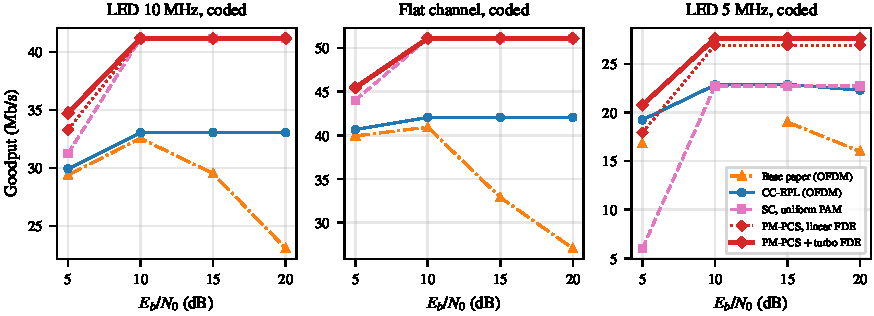
\includegraphics[width=\textwidth]{figures/fig_pm_coded.pdf}
\caption{Coded goodput (CCDM/PAS, irregular LDPC, pilot-based estimation): OFDM chain vs.\ single-carrier chain with linear and turbo frequency-domain equalization. The gap in the base-paper curve (5\,MHz, 10\,dB) means that no code rate decoded.}\label{fig:pmcoded}
\end{figure*}

\section{PM-PCS Results}\label{sec:pmres}
\subsection{Analytical comparison}
Fig.~\ref{fig:pmsweep} and Table~\ref{tab:pmmain} compare PM-PCS with the OFDM schemes on the three channels. Above about 7.5\,dB, where the LED range is the active constraint, PM-PCS is flat at its maximum and exceeds the Gaussian-input bound of clipped DCO-OFDM by \PMboundMin--\PMboundMax\,\% at 15\,dB. This bound applies to the clipped OFDM model of Section~\ref{sec:model}; it is not a general capacity bound for the LED channel. Its gain over CC-EPL at 15\,dB is \PMccFlat\,\% (flat), \PMccLedTen\,\% (10\,MHz LED) and \PMccLedFive\,\% (5\,MHz LED), and over the base paper \PMbaseMin--\PMbaseMax\,\% at 15\,dB and \PMbaseTFmin--\PMbaseTFmax\,\% at 25\,dB, where the base paper's single distribution suffers most from clipping. The shaping itself contributes up to \PMshapeMax\,\% over uniform PAM on the same block; the rest comes from using the range without clipping.

At low $E_b/N_0$ on the band-limited LEDs, CC-EPL is ahead. When power rather than range is the limit, per-subcarrier loading in OFDM exploits the frequency response better than a single equalized block, and CC-EPL leads below \PMcrossTen\,dB (10\,MHz LED) and \PMcrossFive\,dB (5\,MHz LED). Both rates are closed-form, so a transmitter can compute them and pick the better waveform; we call this the regime-adaptive mode. By construction, its analytical rate is the larger of the two. With the turbo equalizer of Section~\ref{sec:turbo} the switch is not needed in our coded tests.


\begin{table}[t]\centering\footnotesize\setlength{\tabcolsep}{2.6pt}
\caption{Analytical throughput (Mb/s): OFDM (base paper, CC-EPL, Gaussian bound) vs.\ single-carrier blocks (uniform PAM, PM-PCS)}\label{tab:pmmain}
\begin{tabular}{@{}lrrrrrrr@{}}\toprule
LED & dB & \cite{pham2026} & CC-EPL & Bound & SC unif. & \textbf{PM-PCS} & vs.\ CC \\\midrule
Flat & 15 & 42.9 & 52.4 & 56.1 & 62.5 & \textbf{64.5} & +23.1 \\
Flat & 25 & 29.6 & 52.3 & 56.1 & 62.5 & \textbf{64.5} & +23.4 \\
10\,MHz & 15 & 39.0 & 43.4 & 45.0 & 50.5 & \textbf{50.5} & +16.2 \\
10\,MHz & 25 & 28.1 & 43.4 & 45.0 & 50.5 & \textbf{50.5} & +16.4 \\
5\,MHz & 15 & 31.7 & 33.4 & 34.3 & 35.0 & \textbf{36.3} & +8.9 \\
5\,MHz & 25 & 24.7 & 33.4 & 34.3 & 35.0 & \textbf{36.3} & +8.9 \\
\bottomrule\end{tabular}\end{table}


\subsection{Waveform validation}
We transmitted 600 blocks per point through the time-domain link with the complex LED response, estimated the channel from 40 pilot blocks, equalized with~\eqref{eq:sinr}'s MMSE filter and measured the bit-metric rate from the LLRs. Over \PMvalCases\ combinations of channel, $E_b/N_0$ and scheme the measured rate is within \PMvalMaxDev\,\% of the analytical one, and no sample is clipped.

\subsection{Turbo equalization}\label{sec:turbo}
The linear equalizer is what loses to OFDM loading at low $E_b/N_0$ on band-limited LEDs: the MMSE-FDE SINR~\eqref{eq:sinr} is a harmonic mean over the bins, while OFDM loading exploits every bin separately. With decoder feedback this loss can be recovered. We added a frequency-domain soft-interference-cancellation equalizer: the LDPC decoder's extrinsic output gives soft estimates $\bar x[n]$ with average variance $\bar v$, and
\begin{equation}
\hat x=\bar x+\frac{1}{\mu}\,\mathrm{IDFT}\big\{W_k\,(Y_k-H_k\bar X_k)\big\},\quad W_k=\frac{\bar v H_k^*}{\bar v|H_k|^2+\sigma_k^2},\label{eq:turbo}
\end{equation}
with $\mu=\frac1N\sum_kW_kH_k$, gives estimates that do not depend on a sample's own soft value. Without feedback ($\bar x=0$, $\bar v=P_s$) this is the MMSE-FDE; with perfect feedback it reaches the matched-filter bound $\mathrm{SINR}=\frac1N\sum_k\rho^2|H_k|^2P_s/\sigma_k^2$, which by Jensen's inequality is never worse than what OFDM loading can use. We checked both limits numerically. The receiver alternates equalization and decoding up to six times. With our LDPC codes the gain appears where the decoder makes partial progress: above the threshold of the linear receiver a failed decode returns almost no extrinsic information, so the loop cannot start.

\subsection{Coded goodput}
The coded chain reuses the LDPC code library, frame length ($N_c=32256$), pilot overhead ratio (one pilot block per eight data blocks) and goodput accounting of Section~\ref{sec:pas}, and the OFDM chain was extended to the 5\,MHz LED for this comparison. Amplitudes come from a constant-composition distribution matcher over 384 symbols with exact multiset ranking, so the 8-point shapes are realized exactly. The receiver estimates the channel from binary pilot blocks, equalizes in the frequency domain and computes Gray-labelled bit LLRs. Every single-carrier scheme, PM-PCS included, is designed once for 4 and once for 8 points and keeps the better of the two in measured goodput, just as every OFDM scheme keeps its best code rate and profile; this keeps a weakness of our LDPC codes on one PAM order from deciding the comparison.

Table~\ref{tab:pmcoded} and Fig.~\ref{fig:pmcoded} show the result for 12 operating points (three channels, $E_b/N_0=5$, 10, 15 and 20\,dB), with 40 frames per code rate. PM-PCS with turbo equalization has the highest goodput at all 12 points; at the six points from 10 to 20\,dB on the flat and 10\,MHz channels it is tied with uniform single-carrier PAM. It is \PMcodedLowMin\ to \PMcodedLowMax\,\% above CC-EPL at 5\,dB and \PMcodedCCmin--\PMcodedCCmax\,\% above it between 10 and 20\,dB, and \PMcodedBaseMin--\PMcodedBaseMax\,\% over the base paper at 15 and 20\,dB. The turbo equalizer adds up to \PMturboFive\,\% at 5\,dB and is what turns the 5\,MHz LED at 5\,dB, the point where linear PM-PCS loses to OFDM loading, into a gain.

The shaping part behaves differently on the three channels. On the flat and 10\,MHz channels PM-PCS is between \PMcodedShapeMin\,\% and \PMcodedShapeMax\,\% of the best single-carrier baseline: uniform 4-PAM already reaches the highest code rate of the library (0.9) on the flat channel, and our IRA codes cannot exploit the extra points of the 8-point optimum. On the 5\,MHz LED the peak-matched constellation gains \PMcodedShapeFiveMin\,\% over the best single-carrier baseline from 10 to 20\,dB, and at 5\,dB the uniform and MB constellations reach only \PMcodedSCfive\,Mb/s, so there the shaping is what makes the single-carrier link work at all.

\begin{table}[t]\centering\footnotesize\setlength{\tabcolsep}{2.6pt}
\caption{Coded goodput (Mb/s), 40 frames per code rate: OFDM chain (\cite{pham2026}, CC-EPL) vs.\ single-carrier chain with linear and turbo equalization}\label{tab:pmcoded}
\begin{tabular}{@{}lrrrrrrr@{}}\toprule
LED & dB & \cite{pham2026} & CC-EPL & SC unif. & PM-PCS & \textbf{+turbo} & vs.\ CC \\\midrule
10\,MHz & 5 & 29.4 & 29.9 & 31.2 & 33.3 & \textbf{34.7} & +16.0 \\
10\,MHz & 10 & 32.6 & 33.0 & 41.2 & 41.2 & \textbf{41.2} & +24.6 \\
10\,MHz & 15 & 29.5 & 33.1 & 41.2 & 41.2 & \textbf{41.2} & +24.6 \\
10\,MHz & 20 & 23.1 & 33.0 & 41.2 & 41.2 & \textbf{41.2} & +24.6 \\
Flat & 5 & 39.9 & 40.7 & 44.0 & 45.5 & \textbf{45.5} & +11.8 \\
Flat & 10 & 40.9 & 42.1 & 51.1 & 51.1 & \textbf{51.1} & +21.5 \\
Flat & 15 & 32.9 & 42.1 & 51.1 & 51.1 & \textbf{51.1} & +21.5 \\
Flat & 20 & 27.1 & 42.1 & 51.1 & 51.1 & \textbf{51.1} & +21.5 \\
5\,MHz & 5 & 16.8 & 19.2 & 6.0 & 17.9 & \textbf{20.8} & +8.0 \\
5\,MHz & 10 & -- & 22.8 & 22.7 & 26.9 & \textbf{27.6} & +21.0 \\
5\,MHz & 15 & 19.0 & 22.9 & 22.7 & 26.9 & \textbf{27.6} & +20.7 \\
5\,MHz & 20 & 16.0 & 22.3 & 22.7 & 26.9 & \textbf{27.6} & +23.9 \\
\bottomrule\end{tabular}
\vspace{1mm}\\\footnotesize ``--'': no code rate decoded (PAS needs rate $\ge 1/2$).\end{table}


\subsection{Circuit level}
The same ngspice circuit as in Section~\ref{sec:spice} carries the single-carrier blocks (with cyclic prefix) unchanged. PM-PCS loses \PMspLossMin--\PMspLossMax\,\% against its analytical rate, mainly at the band edge: the component at exactly 20\,MHz, which OFDM does not use, depends on the sampling phase and the anti-alias filter. We also measured the circuit's distortion directly by driving it with 4-PAM blocks of increasing peak amplitude: from no signal to the full $\pm400$\,mA swing the residual after channel estimation rises by only about 3\,\% above the noise level, so the LED's nonlinearity is not a significant loss in this circuit. An earlier version of our receiver used a brick-wall anti-alias filter at exactly $B$; its ringing across block boundaries cost up to 0.7\,dB at the band edge, for OFDM as well, and was replaced by a smooth filter with blind timing recovery (Section~\ref{sec:spice}). With this receiver, the uncoded bit-metric rate of PM-PCS through the circuit with droop is \PMspCCmin--\PMspCCmax\,\% above CC-EPL from 10 to 25\,dB and the base paper's Algorithm~1 by up to \PMspBaseMax\,\% (Table~\ref{tab:pmspice}, Fig.~\ref{fig:pmspice}); at 5\,dB the difference is \PMspFive\,\%. With the full coded chain through the circuit, PM-PCS delivers \PMspCodedFifteen\,Mb/s at 15\,dB and \PMspCodedTwenty\,Mb/s at 20\,dB, which is \PMspCodedCCFifteen\,\% and \PMspCodedCCTwenty\,\% relative to CC-EPL and \PMspCodedBaseFifteen\,\% and \PMspCodedBaseTwenty\,\% relative to the base paper's Algorithm~1 on the same circuit.

\begin{figure}[t]\centering
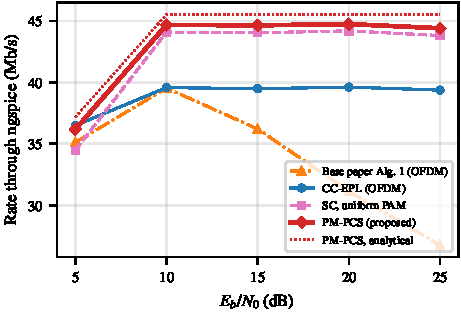
\includegraphics[width=\columnwidth]{figures/fig_pm_spice.pdf}
\caption{Rate through the ngspice circuit with droop: OFDM schemes vs.\ single-carrier blocks.}\label{fig:pmspice}
\end{figure}

\begin{table}[t]\centering\footnotesize\setlength{\tabcolsep}{3.2pt}
\caption{Rate through the ngspice circuit with droop (Mb/s); the first three columns are OFDM}\label{tab:pmspice}
\begin{tabular}{@{}rrrrrrr@{}}\toprule
dB & Alg.~1~\cite{pham2026} & \cite{ling2020} & CC-EPL & SC unif. & \textbf{PM-PCS} & vs.\ CC \\\midrule
5 & 35.1 & 35.4 & 36.5 & 34.5 & \textbf{36.2} & -0.8 \\
10 & 39.5 & 38.4 & 39.6 & 44.1 & \textbf{44.7} & +12.9 \\
15 & 36.2 & 38.1 & 39.5 & 44.0 & \textbf{44.6} & +13.1 \\
20 & 31.2 & 38.3 & 39.6 & 44.2 & \textbf{44.8} & +13.0 \\
25 & 26.7 & 38.2 & 39.4 & 43.8 & \textbf{44.4} & +12.8 \\
\bottomrule\end{tabular}\end{table}


\section{Discussion and Limitations}\label{sec:disc}
\textit{Where the gains come from.} For CC-EPL most of the improvement over~\cite{pham2026} comes from choosing the operating point, which clipping-aware power allocation~\cite{ling2020} already does for uniform QAM; shaping adds a modest \GainPOmin--\GainPOmax\,\% on top. For PM-PCS the gain comes from changing the waveform so that the LED range is used without clipping; the peak-matched shaping adds up to \PMshapeMax\,\% analytically on top of uniform PAM on the same block, and in measured goodput it is worth \PMcodedShapeFiveMin\,\% on the 5\,MHz LED but nothing on the other two channels, where our codes cap it (Section~\ref{sec:pmres}). We consider these the appropriate figures to quote. The main qualitative observation is that the optimized shaping followed the active constraint: MB-like under an average-power limit, few-point and edge-heavy under a range limit. In clipped DCO-OFDM, the subcarrier shaping could not act on the range limit directly.

\textit{The best scheme depends on the metric.} In the analytical model, CC-EPL leads the OFDM schemes at every tested point, while PM-PCS leads CC-EPL except at low $E_b/N_0$ on the band-limited LEDs. In coded goodput, PM-PCS with turbo equalization is highest or tied at all 12 points, but its shaping gain over uniform single-carrier PAM appears only on the 5\,MHz LED. Within OFDM, the coded margin of CC-EPL over coupled power loading is small: a repeated run on the 10\,MHz LED with 80 new frames reduced it to 1.3--2.6\,\%, and through the circuit, with 12 frames per rate, coupled power loading was marginally ahead at 15\,dB. These small coded margins are within the resolution of the tests and should not be read as conclusive.

\textit{Fairness.} PM-PCS uses the same bandwidth, sample rate, cyclic prefix, LED range, noise, power budget, code library and pilot ratio as the OFDM schemes, and it does not use the 100\,mA of headroom above the bias that clipped OFDM does use. It does use all $N=128$ real dimensions of a block, whereas DCO-OFDM leaves the DC bin (bias) and the Nyquist bin empty and uses 126; this is a 1.6\,\% advantage, well below the reported gains, and in the ngspice results the Nyquist bin contributes little. In the coded tests every single-carrier scheme keeps the better of its 4- and 8-point design.

\textit{Limitations.} All results come from simulation; none has been measured on a physical LED link. The analysis of CC-EPL uses the base paper's Bussgang/Gaussian model; the time-domain and ngspice simulations support it for $N=128$. With a linear equalizer PM-PCS loses to OFDM loading on strongly low-pass channels at low $E_b/N_0$; the turbo equalizer removes this in our coded tests, but it costs several decoder passes, and a transmitter without it should use the regime-adaptive mode. The ngspice LED parameters are generic rather than fitted to a measured LED, and its measured distortion is small; a real LED with stronger nonlinearity would hurt the full-range PM-PCS signal more than the clipped OFDM signal, and our circuit cannot rule that out. The LDPC codes are our own irregular IRA codes, about 1.5\,dB from capacity at rate 1/2, with an 8-PAM weakness at low rates; a better code would raise all schemes. PAS cannot go below code rate $(m-1)/m$, which restricts shaping at low $E_b/N_0$. Finally, both schemes need the channel response, and CC-EPL also the clipping parameters, although Fig.~\ref{fig:rob}(b) shows that it is not very sensitive to errors in the latter.

\section{Conclusion}
This report re-implemented a 2026 PCS optimization for clipped DCO-OFDM and found that its printed clipping-noise expression overstates the gain; with the corrected expression, the gain over uniform 16-QAM at 15\,dB is \PCSgainCorrect\,\%. Within OFDM, CC-EPL improved on the base paper and on clipping-aware power loading in the analytical model, but came within a few percent of the Gaussian-input bound, so the room for further shaping gains in this clipped OFDM model is small. Moving the shaping to a DFT-spread block (PM-PCS) allowed the constellation to be designed for the LED range directly, and in our simulations this gave larger gains than further OFDM optimization. The main limitation is that all results come from simulation, including a circuit model with a generic LED; a stronger LED nonlinearity could reduce the advantage of the full-range PM-PCS signal. The most important next step is a measurement on a physical LED link.

% Acknowledgement of tool use -- check your course policy and uncomment if required:
% \section*{Acknowledgement}
% Parts of the simulation code and the text were developed with the help of an AI assistant (Claude, Anthropic); all results were generated by the code in the accompanying project and checked by the author.

\bibliographystyle{IEEEtran}
\bibliography{refs}
\end{document}
